\chapter{Features of the combustion process}
\label{cha:characteristics_of_process}
% \cite{waste_prof} provides a model for describing the combustion process in a plant. However, according to \cite{Elisa_source}, the model suffers from being imprecise. Especially in regards to the lag of the model, as it was described as being too fast. As a result, the mathematical model can not be used directly. Still, by looking at how the system responds to certain step-inputs, some properties of the system can still be inferred. 


\section{Input step-responses}
\begin{figure}[!ht]
    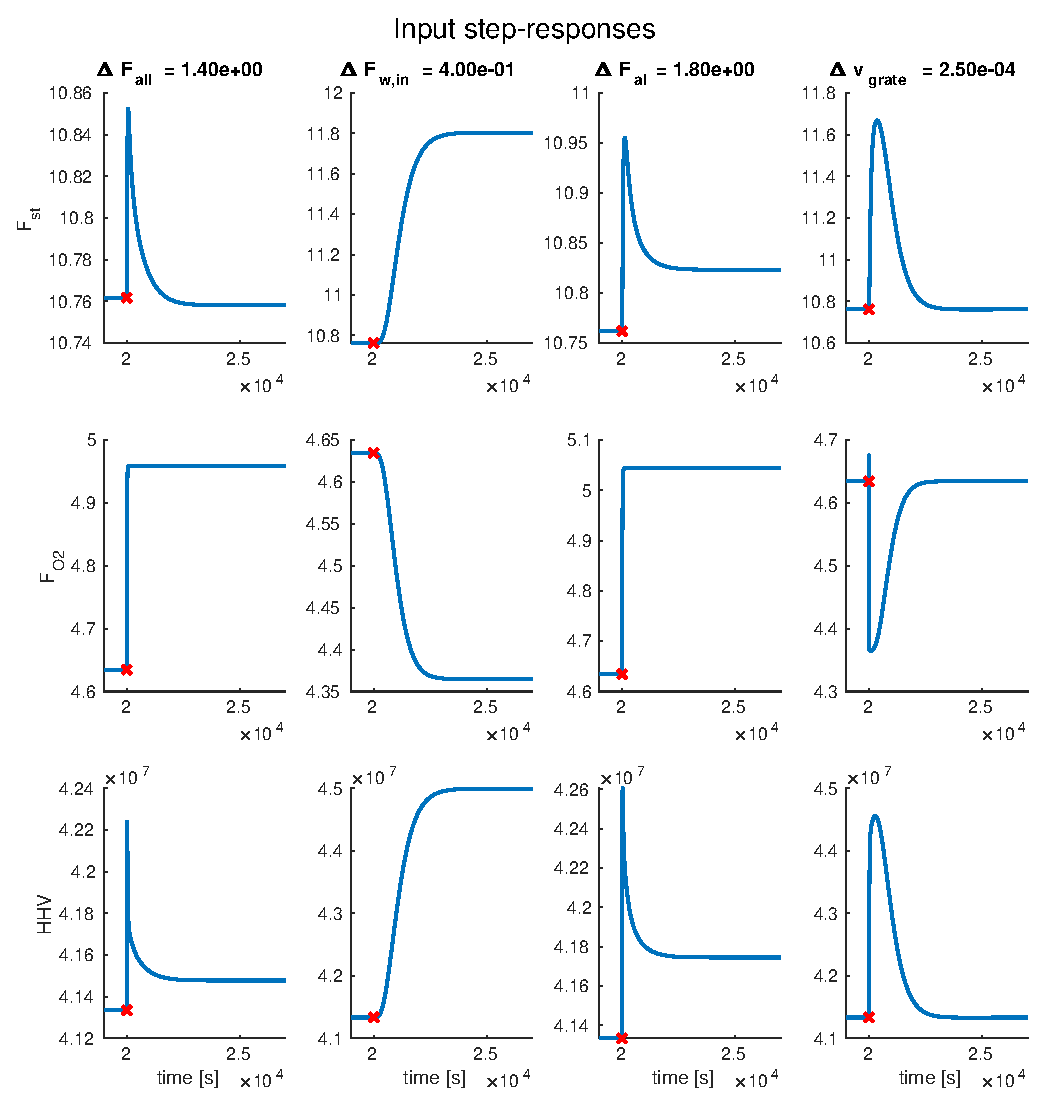
\includegraphics[width=\textwidth]{img/Simple_analysis_plots/Unscaled_input_step_responses.eps}
    \caption{Step-response form the Maniplulable inputs}
    \label{fig:Input_step_response}
\end{figure}

Before doing some actual system identification, it might be useful to do some experiments to get an overview of how the system behaves, as it might give some intuition as to how to control the plant. Figure \ref{fig:unscaled_Input_step_response} shows the result of an experiment  where the first 19000 seconds were used to allow the plant to reach a stationary point, while a constant input-value was held, without any disturbances. At 20000 seconds, one of the input-variables is increased. The point at which the step occurs is shown as a red cross on the graph. Both the inputs and the outputs operate at completely different operating points, and with at completely different orders of magnitude. To better illustrate what is going on, figure \ref{fig:Input_step_response} shows a scaled version of the step-response, where the operating point has been subtracted and the output have been scaled to correspond to what "would have been" if the step-amplitudes had been unity instead. 

\todo[inline]{Different formulation than Manipulable (?)}
\begin{figure}[!ht]
    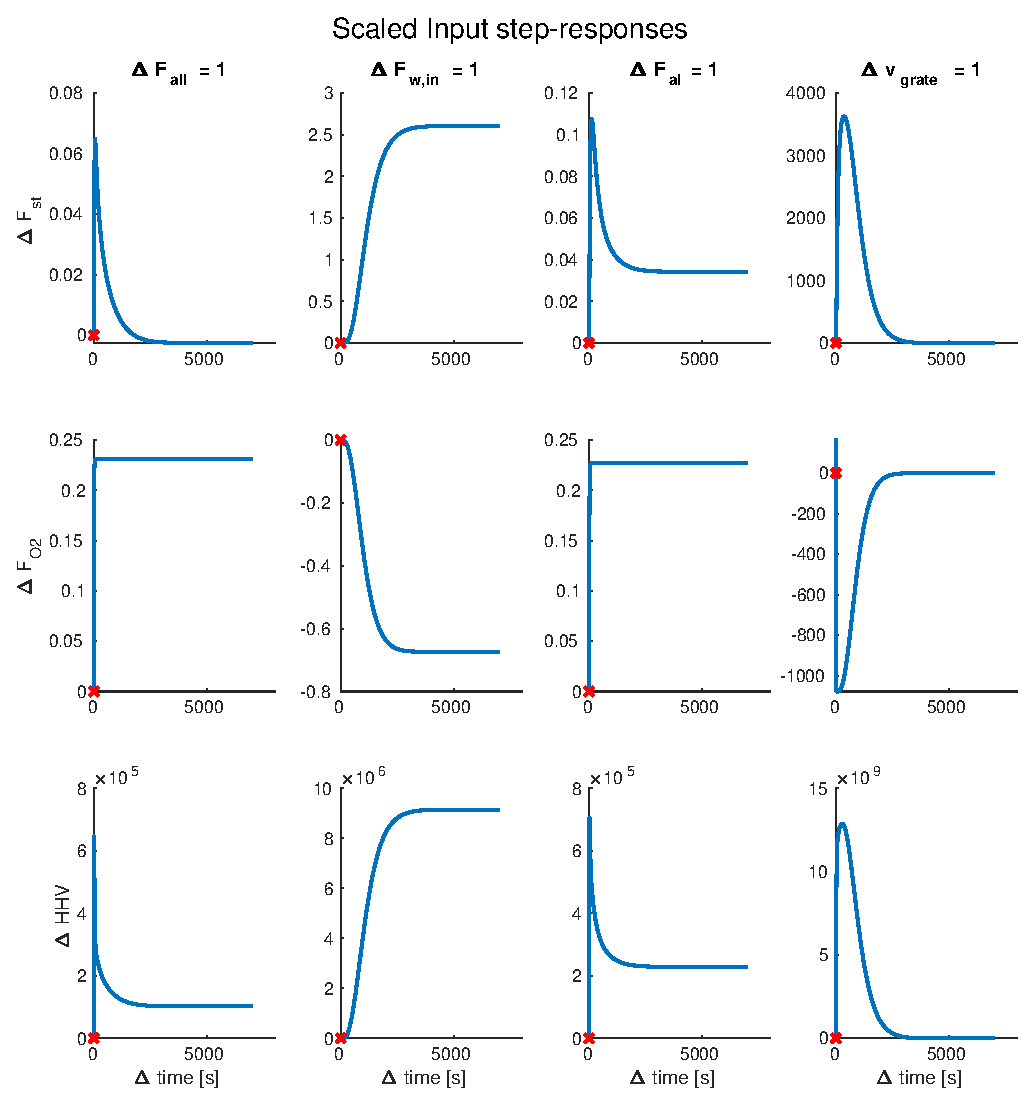
\includegraphics[width=\textwidth]{img/Simple_analysis_plots/Scaled_input_step_responses.eps}
    \caption{Change in outputs, given step-changes in the inputs. Adjusted for the operating point, and scaled for the step-amplitude}
    \label{fig:unscaled_Input_step_response}
\end{figure}

\noindent
As can be seen from figure \ref{fig:Input_step_response}, the speed at which the plant reacts with is very different, depending on the input and the output. The steam-production normally reacts rather slowly to any changes in the amount of waste fed into the plant. This is usually in the realm of thousands of seconds. On the other hand, changing the input of primary or secondary air works almost instantaneously on the mass-flow of air, while also having a fast effect on the steam-production. 

\noindent
The primary air is already pre-heated. Additionally, an increased flow of oxygen flowing through the waste also helps to make more oxygen available for the primary combustion process, which speeds up the process. \cite{Elisa_source} explains that increasing oxygen concentration increases the reaction rate. The effect rapidly decreases again, as the available waste/gases are "used up". 
\noindent

\todo[inline]{@@@ Refer to the article for why the secondary air helps}
\cite{summer_student} suggested that the change in steam-production might have something to do with the fact that any increase in air-flow will also increase the rate at which flue gas moves through the passes. Since it takes some time before the gas moves through the passes, it is possible that the increase comes from old, already heated gas, which moves past the heat-exchange elements at a faster rate, but with the same temperature. This would result in more power being delivered. 
\todo[inline]{Remove everything up to the previous todo /|}

Since more cold air is added to the new flue gas, the result will be that it gets more diluted, and the temperature will drop somewhat as a result. The result will be that the delivered power will go back to roughly the old amount. 
\noindent
It is worth noting that the plant is very sensitive to changes in $v_{\text{grate}}$. This is because it is normally only made to operate at a couple millimetres per second. As a result, it is desirable to only perform small changes to the grate speed. Changing the grate speed still has some advantages. The biggest one is the fact that both the steam-production and the oxygen concentration react a lot more quickly to changes in the grate speed than in the amount of waste fed into the plant. Because of this, one aspect where a model-based controller might be able to improve a bit is in its use of the grate-speed. The air-flows are good for controlling steam-production on a short time-horizon. Changing the waste-flow is good when controlling over a long time-horizon. The grate speed may therefore be used to supplement both of these, by helping to control the steam production over a medium time-horizon. 
\noindent

\section{Disturbance step-responses}


\begin{figure}[!ht]
    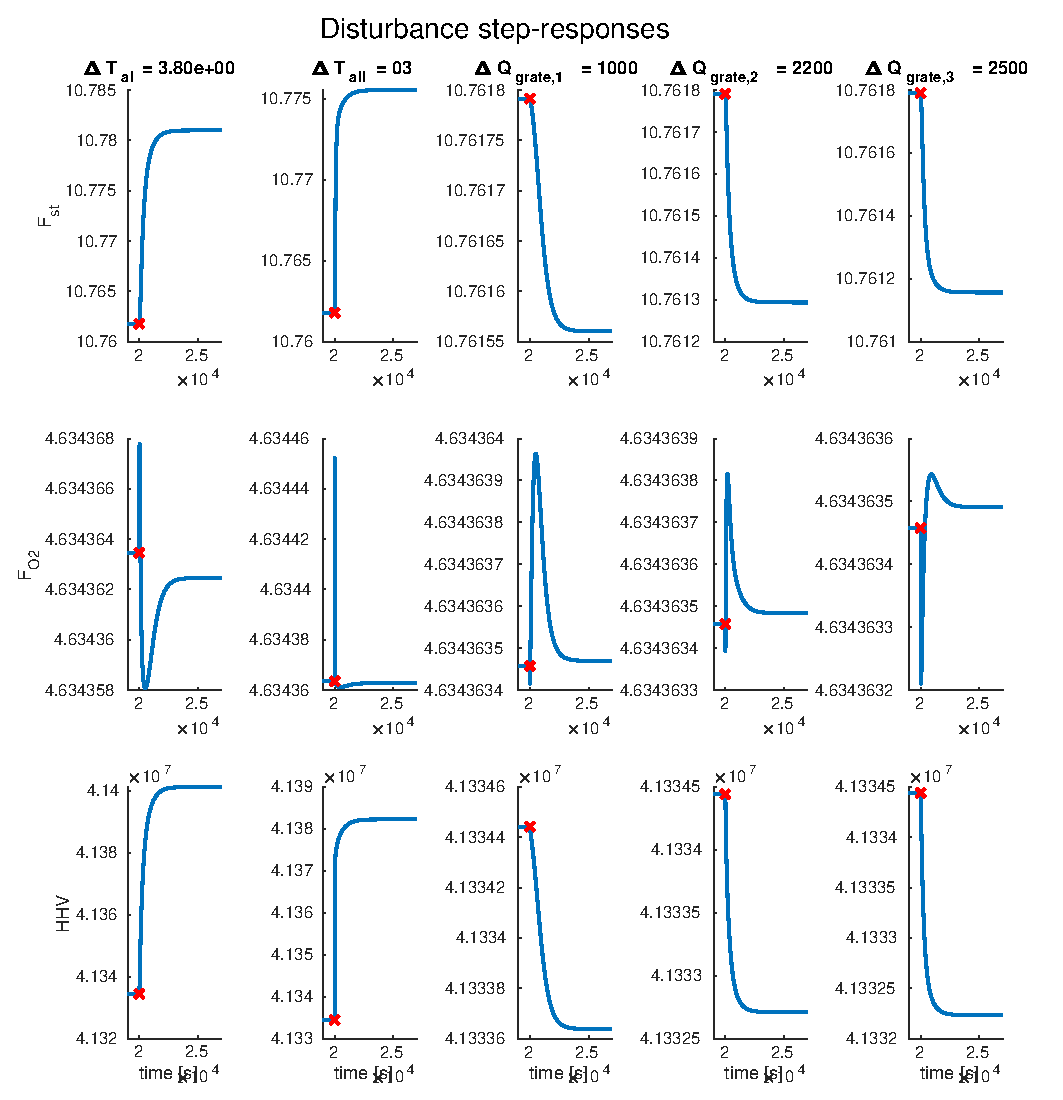
\includegraphics[width=\textwidth]{img/Simple_analysis_plots/Unscaled_disturbance_step_responses.eps}
    \caption{Step-response to the different kinds of disturbances}
    \label{fig:Unscaled_disturbance_response}
\end{figure}

The first two columns in figure \ref{fig:Unscaled_disturbance_response} show the effects of changes in the temperature of the primary and secondary air flow. The three different $Q_{\text{grate}}$ variables represent heat-exchange in the different sections of the grate. In practice, there should also be other variables as well, to represent sudden changes in the concentration of combustible materials or moisture in the waste. But the disturbances that are there show a few very interesting points. The first observation is the small effect that air-temperature has on the steam-production. Figure \ref{fig:Scaled_disturbance_response} show that a change of one degree in the temperature of the primary or secondary air will only change the steam-production by $4 \left[ \frac{kg}{s} \right]$. On the other had, the three values for $Q_{\text{grate}}$ fluctuate more in the range of $10^4$, so all changes in air temperature become completely dominated by the disturbances from $Q_{\text{grate}}$. Because of this, the disturbances resulting from changes in air temperature will not be taken into consideration when designing controllers.
\todo[inline]{Should there be another form of disturbance instead?}
\noindent
Finally, the biggest takeaway from plotting the disturbances can be seen when looking at the effects both of them have on $F_{O2}$. As a result, the disturbances almost entirely affect the production of steam, while most changes to the mass-flow of air in the flue gas are a result of the attempts to correct the disturbances. This means that a feed-forward controller that tries to cancel the effects of $Q_{\text{grate}}$ can only focus on the steam-production, and then another feed forward controller can be used to negate the changes in $F_{O2}$ that result from trying to correct for the changes in $F_{st}$


\noindent

\todo[inline]{Add this section}

\begin{figure}[!ht]
    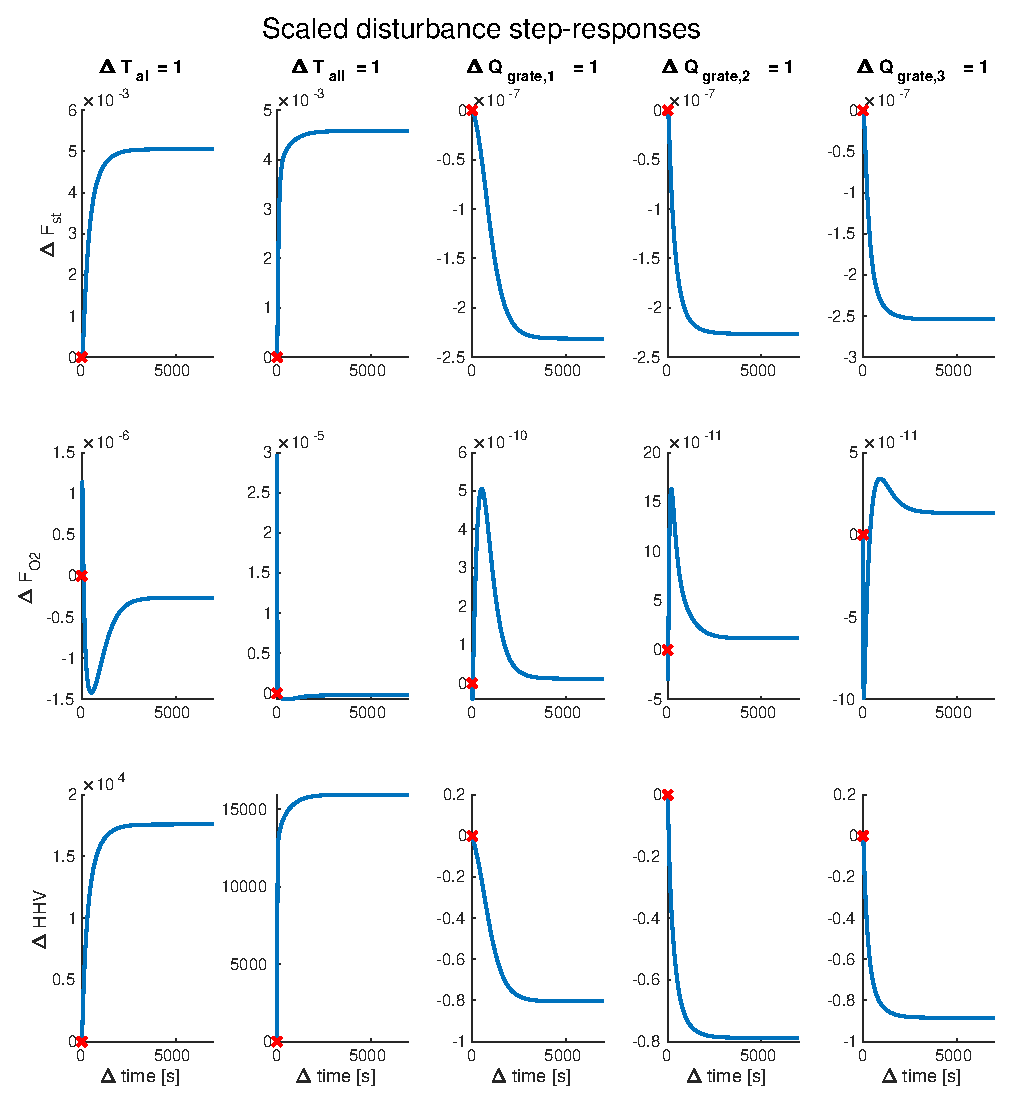
\includegraphics[width=\textwidth]{img/Simple_analysis_plots/Scaled_disturbance_step_responses.eps}
    \caption{Change in outputs, given step-changes in the the disturbances. Adjusted for the operating point, and scaled for the step-amplitude}
    \label{fig:Scaled_disturbance_response}
\end{figure}
\todo[inline]{Add units to the plots. Oxygen is [?/s], while HHV is [J/s]}



\section{Some observations}

\subsection{Justifying the use of an HHV-estimator}

When looking at figures \ref{fig:unscaled_Input_step_response} and \ref{fig:Unscaled_disturbance_response}, it can be seen that $F_{st}$ and $\hat{HHV}$ are remarkably similair, except for their amplitude. Since $F_{st}$ is one of the controlled outputs, the question becomes why $\hat{HHV}$ is necessary. 
\begin{figure}[!ht]
    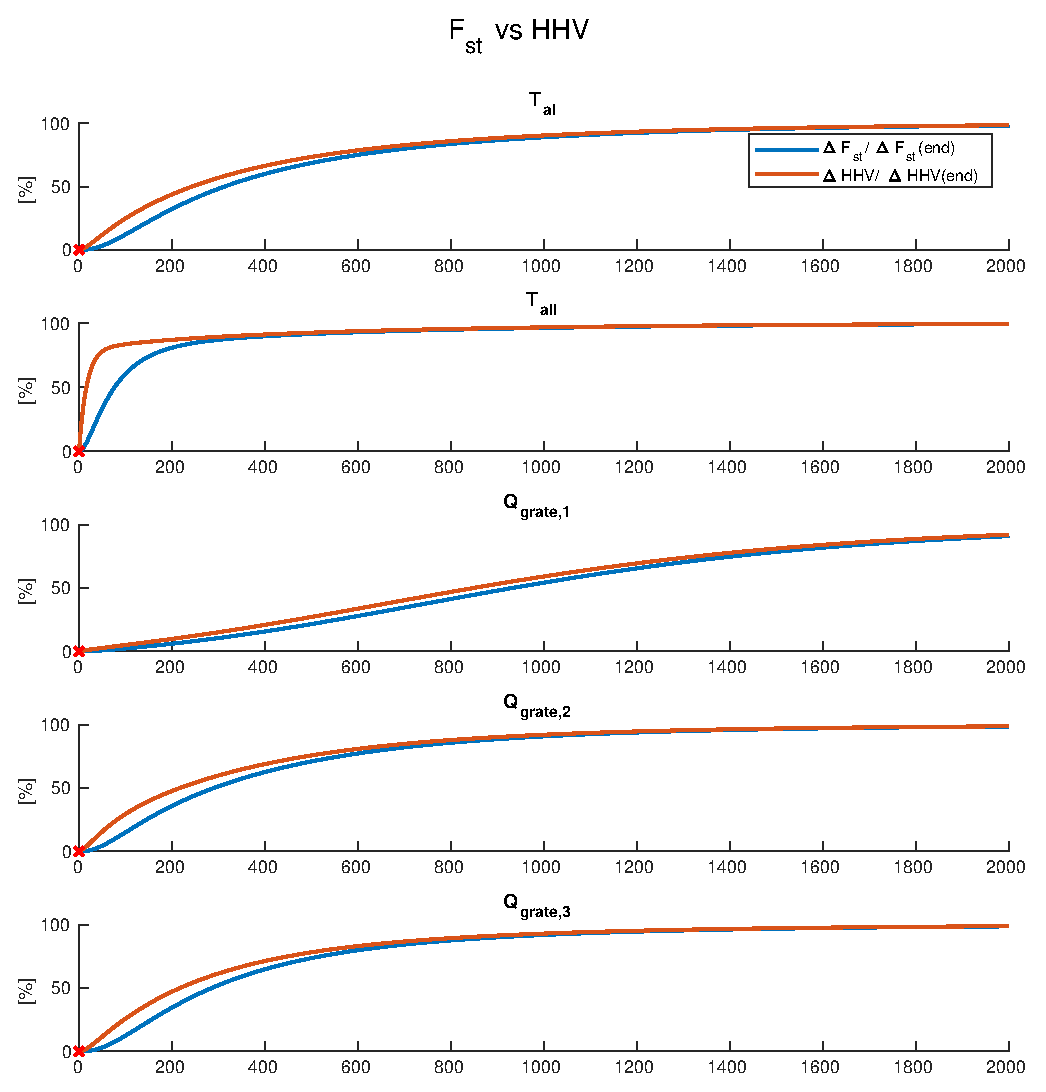
\includegraphics[width=\textwidth]{img/Simple_analysis_plots/Compare_F_st_to_HHV.eps}
    \caption{Change in $\hat{HHV}$ and $F_{st}$ as percentage of total change. Given as percentage to make them comparable.}
    \label{fig:F_st_vs_HHV}
\end{figure}
\noindent
Figure \ref{fig:F_st_vs_HHV} shows the step-responses of  $F_{st}$ and $\hat{HHV}$, without the mean, and represented as percentage of the infinite-horizon change. The two plots are very similair, but $F_{st}$ lags behind $\hat{HHV}$ by about a minute. In the case of PID-controller, this opens up for using a cascaded PID-controller, as was done in \cite{summer_student}, which allows for higher bandwidht, while also keeping the robustness of the previous controller. A model-based controller will be able to use the extra measurement of $\hat{HHV}$ to detect any changes in plant-disturbances earlier, but also to as a means to mitigate the effects of measurement-noise, as long as the two measurements are uncorrolated. 

\subsection{Usage of air when controlling steam production}

The results that will be discussed in section \ref{sec:MPC_results} show that some controllers will attempt to primarily use air to control the steam-production around the operating point. This is normally bad, but the way it is done is somewhat interesting. Instead of using $F_{aI}$, like it has been done in the previous controllers, it instead uses $F_{aI} -F_{aII}$ to increase the production of steam. There are two main reasons for doing this. Primarily, because changing $F_{aI}$ - $F_{aII}$  does not affect the total amount of oxygen added to the flue gas, leading to fewer changes in $F_{O2}$. The second reason can be seen in figure \ref{fig:F_diff_impulse_response}. By keeping the total amount of oxygen injected into the system constant, the step-response becomes more well-behaved, potentially leading to a controller that can be allowed to be more aggressive. 



\begin{figure}[!ht]
    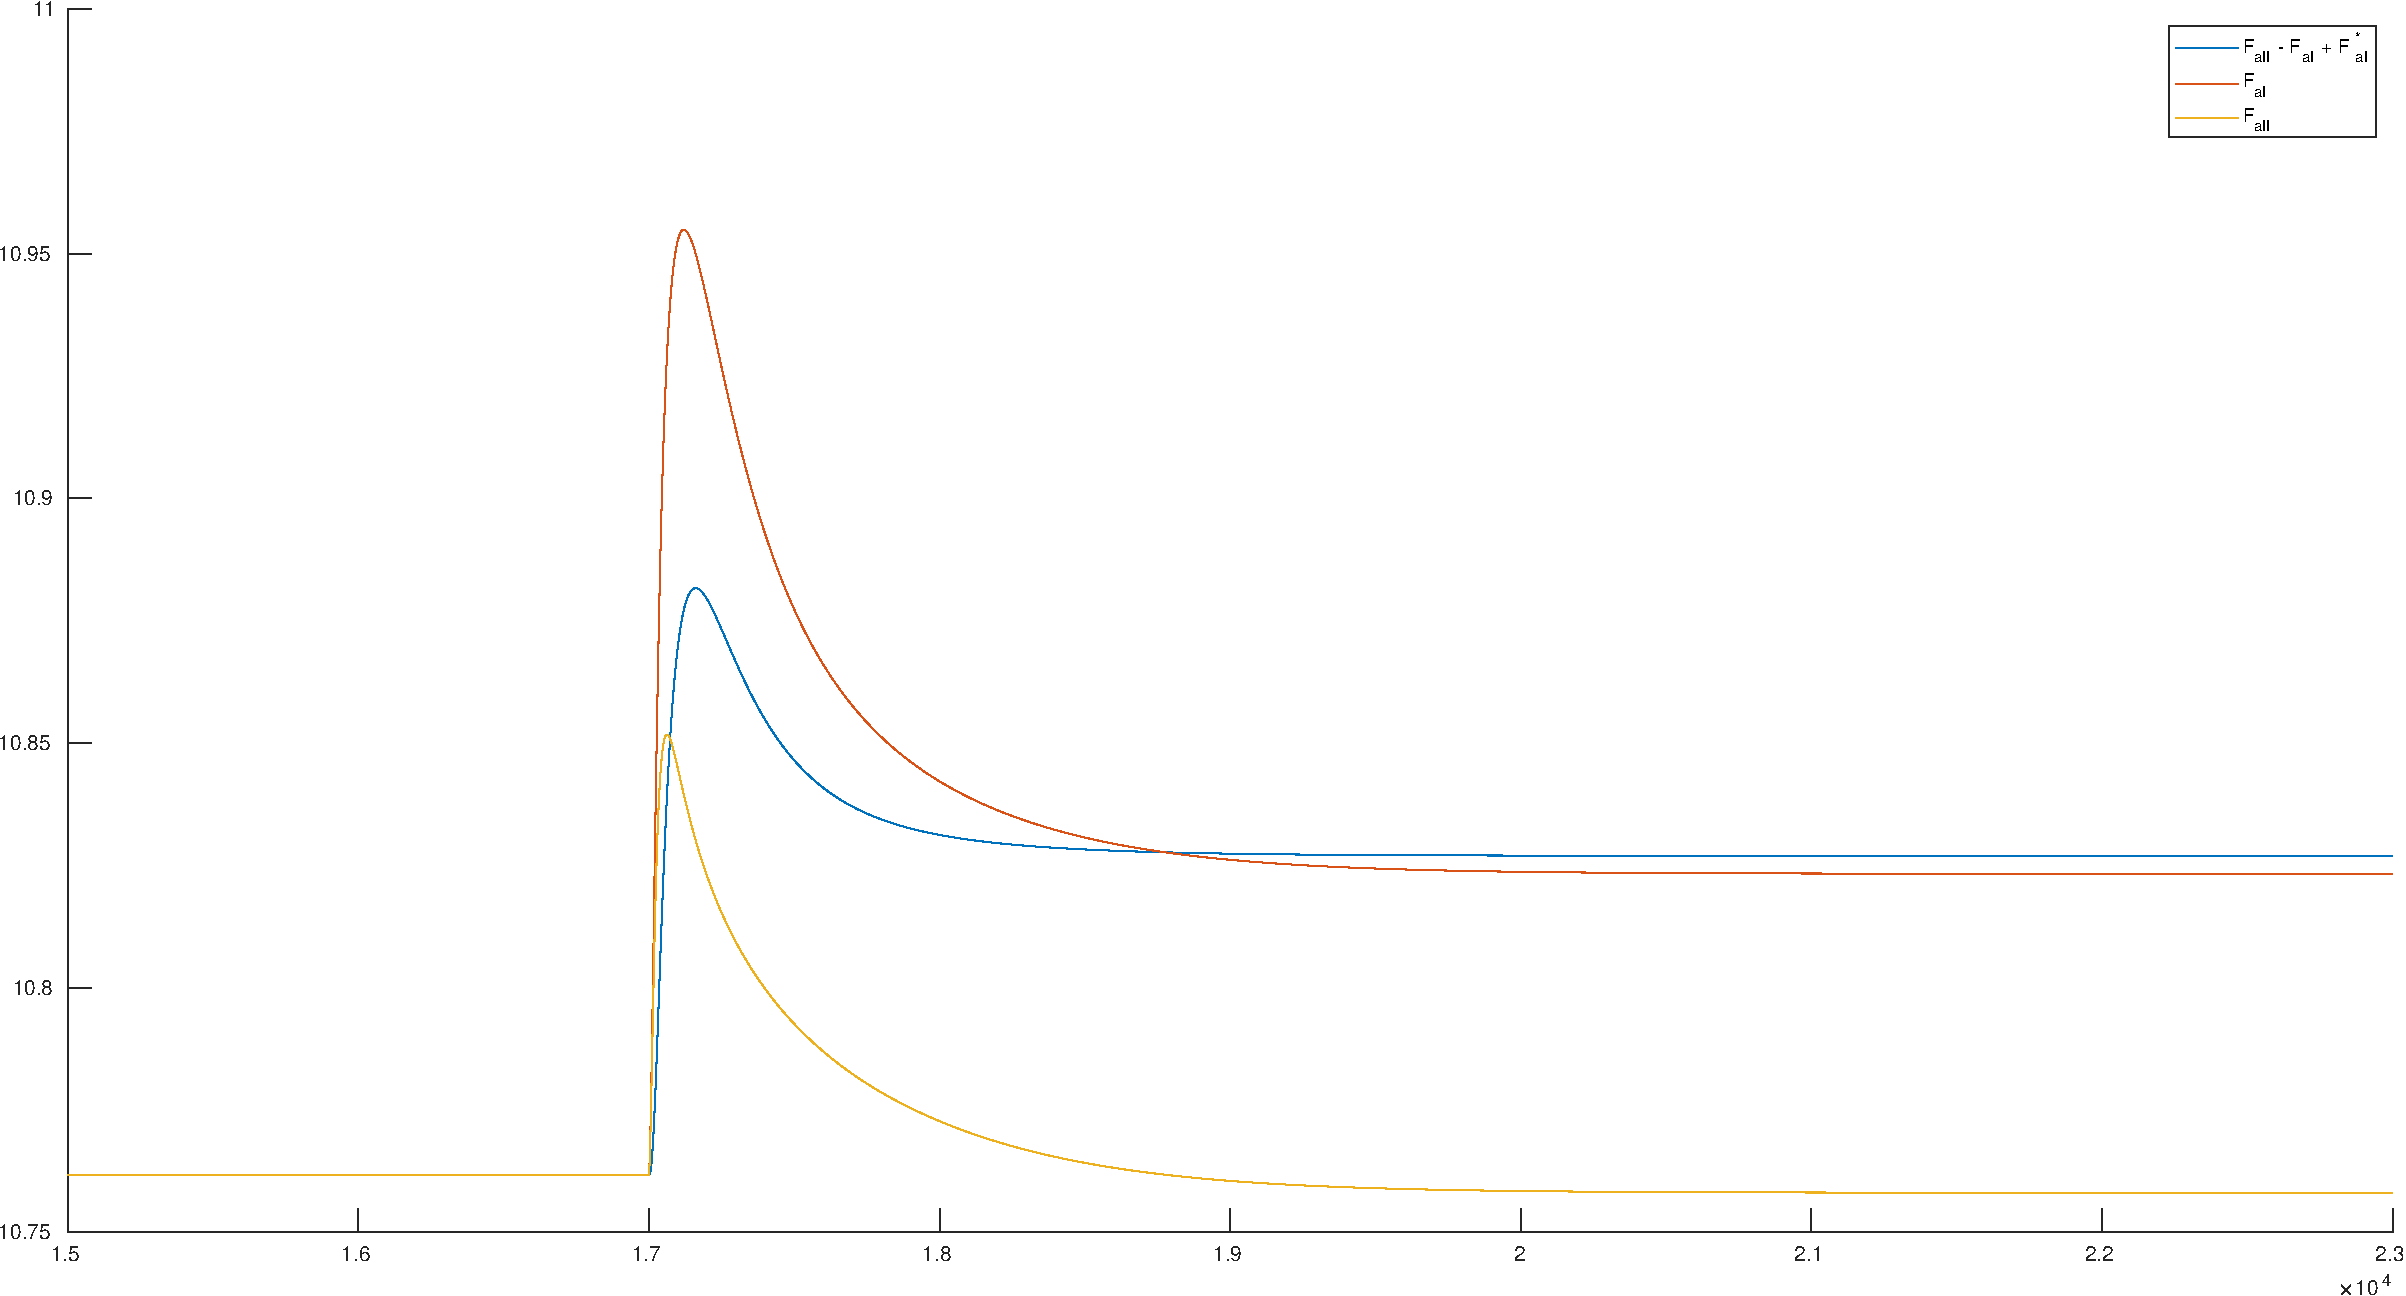
\includegraphics[width=\textwidth]{img/compare_steam_from_air_inputs-eps-converted-to.pdf}
    \caption{Change in outputs, given step-changes in the the disturbances. Adjusted for the operating point, and scaled for the step-amplitude}
    \label{fig:F_diff_impulse_response}
\end{figure}

A PID-controller with this premise was not implemented in this project, but it could potentially be an avenue for further research. 
\todo[inline]{Add this section @@@}
